 \chapter*{Introduction} \label{intro:chapter}
%mbxSTARTIGNORE
\addfakecontentsline{Introduction}
\markboth{INTRODUCTION}{INTRODUCTION}
%mbxENDIGNORE

%%%%%%%%%%%%%%%%%%%%%%%%%%%%%%%%%%%%%%%%%%%%%%%%%%%%%%%%%%%%%%%%%%%%%%%%%%%%%%

\section{Notes à propos de ce manuel}
\label{notes:section}

%\sectionnotes{à propos de l'auteur.}
Ceci est une traduction d'un manuel libre écrit par Ji\v{r}\'{\i} Lebl.  Il s'agit d'un premier cours d'équations différentielles pour les personnes étudiant en génie.

Originalement des notes pour un cours enseigné 
à \href{https://www.math.uiuc.edu/}{University of Illinois
Urbana-Champaign} en 2008-2009, l'auteur  les a utilisées ensuite 
à UIUC\@, \href{https://www.math.ucsd.edu/}{University of California, à San Diego} (UCSD) 
et à \href{https://math.okstate.edu/}{Oklahoma State University} (OSU).
Normalement, ces cours sont enseignés avec le livre de 
Edwards et Penney, \emph{Differential
Equations and Boundary Value Problems: Computing and Modeling}~\cite{EP}, ou celui de Boyce et DiPrima,
\emph{Elementary
Differential Equations and Boundary Value Problems}~\cite{BD},
et ce manuel-ci se veut un remplacement de ces ressources.

L'adaptation en français a été écrite pour les cours de GCH217 et MAT217, donnés à l'Université de Sherbrooke.

Voici d'autres références :
E. L.\ Ince,
\emph{Ordinary Differential Equations}~\cite{I}, classique (et économique);
Stanley Farlow, \emph{An Introduction to Differential Equations and Their
Applications}~\cite{F}; 
Berg et McGregor,
\emph{Elementary Partial Differential Equations}~\cite{BM}, maintenant disponible dans Dover;
et William Trench,
\emph{Elementary
Differential Equations with Boundary Value Problems}~\cite{T}, une ressource libre.
Voir le chapitre \hyperref[furtherreading:chapter]{Lectures additionnelles} à la fin de ce manuel.

%\subsection{Organisation}
%
%L'organisation de ce livre requiert que les chapitres soient abordés dans l'ordre.  Les chapitres de la fin peuvent être omis.  L'interdépendance du contenu est comme suit.
%
%% If changing make sure to also update figures/chapterdiagram.pdf_t
%% That's a hopefully short term hack before I figure out how to do it
%% better so that it also gets links and such
%%mbxSTARTIGNORE
%
%\begin{equation*}
%\begin{tikzcd}[cramped, row sep=small]
%& {\text{\hyperref[intro:chapter]{Introduction}}} \arrow[d] \\
%{\text{\Appendixref{linalg:appendix}}} \arrow[dd, dotted]
%& {\text{\Chapterref{fo:chapter}}} \arrow[d] \\
%& {\text{\Chapterref{ho:chapter}}} \arrow[dddr] \arrow[dd] \arrow[dl] \arrow[dr] \\
%{\text{\Chapterref{sys:chapter}}} \arrow[dr, dotted] \arrow[d] & 
%  {\text{\Chapterref{ps:chapter}}} \\
%{\text{\Chapterref{nlin:chapter}}} & {\text{\Chapterref{FS:chapter}}} \arrow[d]
%\arrow[dr,dotted] \\
%& {\text{\Chapterref{SL:chapter}}}
%& {\text{\Chapterref{LT:chapter}}}
%\end{tikzcd}
%\end{equation*}
%
%%mbxENDIGNORE
%%mbxlatex \begin{center}
%%mbxlatex \inputpdft{chapterdiagram}
%%mbxlatex \end{center}
%
%Les chapitres \ref{FS:chapter} et \ref{SL:chapter} contiennent certaines références au
% \chapterref{sys:chapter} (un peu d'algèbre linéaire), mais ces références ne sont pas essentielles et peuvent être parcourues rapidement.
%Quant au \chapterref{LT:chapter}, il ne dépend pas de \chapterref{FS:chapter} sauf pour la section sur les EDP \ref{laplacepde:section},
%Cependant, en théorie il pourrait être couvert de manière indépendante.
%L'\appendixref{linalg:appendix} couvre de manière plus substantielle l'algèbre linéaire que la section de révision
% \sectionref{sec:matrix}, pour un cours combinant l'algèbre linéaire et les équations différentielles ordinaires\@.

%\medskip
%\subsection{Typical types of courses}
%
%Several typical types of courses can be run with the book.
%There are the two original courses at UIUC\@,
%both cover ODE as well some PDE\@.
%Either, there is the 4 hours-a-week for a semester (Math 286 at UIUC):
%
%\medskip
%
%\noindent
%\hyperref[intro:chapter]{Introduction} (\ref{introde:section}),
%\chapterref{fo:chapter} (\ref{integralsols:section}--\ref{numer:section}),
%\chapterref{ho:chapter},
%\chapterref{sys:chapter},
%\chapterref{FS:chapter} (\ref{bvp:section}--\ref{dirich:section}),
%\chapterref{SL:chapter} (or
%\ref{LT:chapter} or \ref{ps:chapter} or \ref{nlin:chapter}).
%
%\medskip
%
%Or, the second course at UIUC is at 3 hours-a-week (Math 285 at UIUC):
%
%\medskip
%
%\noindent
%\hyperref[intro:chapter]{Introduction} (\ref{introde:section}),
%\chapterref{fo:chapter} (\ref{integralsols:section}--\ref{numer:section}),
%\chapterref{ho:chapter},
%\chapterref{FS:chapter} (\ref{bvp:section}--\ref{dirich:section}),
%(and maybe \chapterref{SL:chapter},
%\ref{LT:chapter}, or \ref{ps:chapter}).
%
%\medskip
%
%A semester-long course at 3 hours a week that doesn't cover either systems or PDE
%will cover, beyond the introduction,
%%\sectionref{introde:section},
%\chapterref{fo:chapter},
%\chapterref{ho:chapter},
%\chapterref{LT:chapter}, and \chapterref{ps:chapter},
%(with sections skipped as above).
%On the other hand, a typical course that covers 
%systems will probably need to skip Laplace and power series
%and cover
%%\sectionref{introde:section},
%\chapterref{fo:chapter},
%\chapterref{ho:chapter},
%\chapterref{sys:chapter}, and \chapterref{nlin:chapter}.
%
%\medskip
%
%If sections need to be skipped in the beginning, a good core of the 
%sections on single ODE is:
%\ref{introde:section},
%\ref{integralsols:section}--\ref{intfactor:section},
%\ref{auteq:section},
%\ref{solinear:section},
%\ref{sec:ccsol},
%\ref{sec:mv}--\ref{forcedo:section}.
%
%\medskip
%
%The complete book can be covered at a reasonably
%fast pace at approximately 76 lectures
%(without \appendixref{linalg:appendix})
%or 86 lectures (with \appendixref{linalg:appendix} replacing
%\sectionref{sec:matrix}).
%This is not accounting for exams, review,
%or time spent in a computer lab. % (if using IODE for example).
%A two-quarter or a two-semester course can be easily run with the material.
%For example (with some sections perhaps strategically skipped):
%
%\medskip
%
%\noindent
%Semester 1:
%\hyperref[intro:chapter]{Introduction},
%\chapterref{fo:chapter},
%\chapterref{ho:chapter},
%\chapterref{LT:chapter},
%\chapterref{ps:chapter}.
%\\
%Semester 2: 
%\Chapterref{sys:chapter},
%\chapterref{nlin:chapter},
%\chapterref{FS:chapter},
%\chapterref{SL:chapter}.
%
%\medskip
%
%A combined course on ODE with linear algebra can run as:
%
%\medskip
%
%\noindent
%\hyperref[intro:chapter]{Introduction},
%\chapterref{fo:chapter} (\ref{integralsols:section}--\ref{numer:section}),
%\chapterref{ho:chapter},
%\appendixref{linalg:appendix},
%\chapterref{sys:chapter} (w/o \sectionref{sec:matrix}), (possibly 
%\chapterref{nlin:chapter}).
%
%\medskip
%
%The chapter on
%the Laplace transform (\chapterref{LT:chapter}),
%the chapter on Sturm--Liouville (\chapterref{SL:chapter}),
%the chapter on power series (\chapterref{ps:chapter}),
%and the chapter on nonlinear systems (\chapterref{nlin:chapter}),
%are more or less interchangeable and can be treated as \myquote{topics}.
%If \chapterref{nlin:chapter} is covered, it may be best to place it right 
%after \chapterref{sys:chapter},
%and \chapterref{SL:chapter} is best covered right after
%\chapterref{FS:chapter}.
%If time is short, the first two sections of
%\chapterref{ps:chapter} make a reasonable self-contained unit.

%%\medskip
%\subsection{Computer resources}
%
%The book's
%website \url{https://www.jirka.org/diffyqs/}
%contains the following resources:
%\begin{enumerate}
%\item Interactive SAGE demos.
%\item Online WeBWorK homeworks
%(using either your own WeBWorK installation or Edfinity)
%for most sections, customized for this book.
%\item The PDFs of the figures used in this book.
%\end{enumerate}
%
%I taught the UIUC courses using IODE\index{IODE software}
%(\url{https://faculty.math.illinois.edu/iode/}).
%IODE is a free software package that
%works with Matlab (proprietary) or Octave (free software).
%%Unfortunately IODE is not kept up to date at this point, and may have
%%trouble running on newer versions of Matlab.
%The graphs in the book were made with
%the Genius\index{Genius software} software
%(see \url{https://www.jirka.org/genius.html}).  I use Genius
%in class to show these (and other) graphs.
%
%The \LaTeX\ source of the book is also available
%for possible modification and customization
%at github (\url{https://github.com/jirilebl/diffyqs}).
%
%%\medskip
%
%%\textbf{Acknowlegements:}
%
%\subsection{Acknowledgments}
%
%Firstly, I would like to acknowledge Rick Laugesen.  I used his handwritten
%class notes
%the first time I taught
%Math 286.  My organization of this book through chapter 5,
%and the choice of
%material covered, is heavily influenced by his notes.  Many
%examples and computations are taken from his notes.  I am also heavily
%indebted to Rick for all the advice he has given me, not just on teaching
%Math 286.
%For spotting errors and other suggestions,
%I would also like to acknowledge (in no particular order):
%John P.\ D'Angelo,
%Sean Raleigh, Jessica Robinson, Michael Angelini, Leonardo Gomes, Jeff
%Winegar, Ian Simon, Thomas Wicklund, Eliot Brenner, Sean Robinson,
%Jannett Susberry, Dana Al-Quadi, Cesar Alvarez, Cem Bagdatlioglu,
%Nathan Wong, Alison Shive, Shawn White, Wing Yip Ho, Joanne Shin,
%Gladys Cruz, Jonathan Gomez, Janelle Louie, Navid Froutan,
%Grace Victorine, Paul Pearson, Jared Teague, Ziad Adwan,
%Martin Weilandt, S\"{o}nmez \c{S}ahuto\u{g}lu,
%Pete Peterson, Thomas Gresham, Prentiss Hyde, Jai Welch,
%Simon Tse, Andrew Browning, James Choi, Dusty Grundmeier,
%John Marriott,
%Jim Kruidenier,
%Barry Conrad,
%Wesley Snider,
%Colton Koop,
%Sarah Morse,
%Erik Boczko,
%Asif Shakeel,
%Chris Peterson,
%Nicholas Hu,
%Paul Seeburger,
%Jonathan McCormick,
%David Leep,
%William Meisel,
%Shishir Agrawal,
%Tom Wan,
%Andres Valloud,
%and probably others I
%have forgotten.
%Finally, I would like
%to acknowledge NSF grants DMS-0900885 and DMS-1362337.
%

%%%%%%%%%%%%%%%%%%%%%%%%%%%%%%%%%%%%%%%%%%%%%%%%%%%%%%%%%%%%%%%%%%%%%%%%%%%%%%

\sectionnewpage
\section{Introduction aux équations différentielles}
\label{introde:section}

%\sectionnotes{more than 1 lecture\EPref{, \S1.1 in \cite{EP}}\BDref{,chapter 1 in \cite{BD}}}

\subsection{Équations différentielles}

Les lois de la physique sont généralement exprimées sous forme d'équations différentielles.  Ainsi, toute discipline de science ou de génie utilise les équations différentielles, à un niveau plus ou moins sophistiqué.  Comprendre les équations différentielles est essentiel à la compréhension de presque tout ce que vous apprendrez dans vos cours de science ou de génie.  On peut penser aux mathématiques comme au langage de la science, et les équations différentielles forment une partie importante de ce langage.
%As an analogy,
%suppose all your classes from now on were given in Swahili.  
%It would be important to first learn Swahili, or you would have a very
%tough time getting a good grade in your classes.

Vous avez déjà vu plusieurs équations différentielles, peut-être sans savoir que c'en était.
Et vous avez même résolu des équations différentielles dans vos cours de calcul.  Voyons un exemple que vous n'avez peut-être pas vu:
\begin{equation} \label{eq1}
\frac{dx}{dt} + x = 2 \cos t .
\end{equation}
Ici, $x$ est la  \emph{\myindex{variable dépendante}}, et $t$ est la \emph{\myindex{variable indépendante}}.
L'équation \eqref{eq1}
est un exemple de base d'une \emph{\myindex{équation différentielle}}. Plus précisément, c'est un exemple d'\emph{\myindex{équation différentielle du premier ordre}}, puisqu'elle n'implique que la première dérivée de la variable dépendante $x$.  Cette équation vient de la loi de refroidissement de Newton, lorsque la température ambiante oscille en fonction du temps.

\subsection{Solutions d'équations différentielles}

Quand on résout une équation différentielle comme \eqref{eq1}, l'inconnue est une variable $x$, qui elle-même dépend d'une variable $t$, c'est-à-dire qu'on veut trouver un $x$, dépendant de $t$, tel que, lorsqu'on substitue $x$, $t$ et $\frac{dx}{dt}$ dans l'équation \eqref{eq1}, le côté gauche est égal au côté droit, et donc l'égalité est satisfaite.  C'est le même principe que pour une équation ordinaire (algébrique) impliquant $x$ et $t$.  Nous affirmons que l'expression suivante est une \emph{\myindex{solution}}: 
\begin{equation*}
x = x(t) = \cos t + \sin t .
\end{equation*}
%
Comment le vérifier?  Il suffit de substituer $x$ dans l'équation \eqref{eq1} et de vérifier que l'égalité est bel et bien établie.    Nous devons d'abord calculer $\frac{dx}{dt}$.  On trouve que $\frac{dx}{dt} = 
-\sin t + \cos t$.  Maintenant, calculons le côté gauche de \eqref{eq1}: 
\begin{equation*}
\frac{dx}{dt} + x = 
\underbrace{(-\sin t + \cos t)}_{\frac{dx}{dt}}
+
\underbrace{(\cos t + \sin t)}_{x}
=
2\cos t .
\end{equation*}
C'est bien ce que nous voulons: nous obtenons exactement le côté droit de l'équation.
Mais ce n'est pas tout. 
Nous affirmons que 
$x = \cos t + \sin t + e^{-t}$ est aussi une solution.  Vérifions: 
\begin{equation*}
\frac{dx}{dt} = -\sin t + \cos t - e^{-t} .
\end{equation*}
On remplace ceci dans \eqref{eq1}: 
\begin{equation*}
\frac{dx}{dt} + x = 
\underbrace{(-\sin t + \cos t - e^{-t})}_{\frac{dx}{dt}} +
\underbrace{(\cos t + \sin t + e^{-t})}_{x}
= 2\cos t .
\end{equation*}
Il s'agit bien d'une solution.

Ainsi, plusieurs solutions sont possibles.  Pour cette équation en particulier, toutes les solutions peuvent s'écrire sous la forme 
\begin{equation*}
x = \cos t + \sin t + C e^{-t} 
\end{equation*}
pour une constante $C$.  Différentes constantes $C$ donneront des solutions différentes, donc il y a vraiment un nombre infini de solutions possibles.  Voir la~\figurevref{intro:plotsfig} pour le graphe de quelques solutions.  Nous verrons un peu plus tard comment trouver ces solutions de manière générale.

\medskip

\begin{mywrapfig}{3.25in}
\capstart
\diffyincludegraphics{width=3in}{width=4.5in}{intro-plots-alt}
\caption{Quelques solutions de $\frac{dx}{dt} + x = 2 \cos t$.\label{intro:plotsfig}}
\end{mywrapfig}%

La résolution d'une équation différentielle peut être très ardue.  Il n'y a pas une méthode générale pour les résoudre toutes. La plupart du temps, nous verrons comment obtenir des formules exactes pour résoudre certaines équations différentielles, mais parfois nous n'obtiendrons que des solutions approximatives. De plus, nous passerons un peu de temps à comprendre certaines équations, sans les résoudre.

La majeure partie de ce manuel est dédiée aux 
\emph{équations différentielles ordinaires\index{ordinary differential equation}},
ou EDO\index{ODE}, c'est-à-dire aux équations ayant une seule variable indépendante, où les dérivées se prennent en termes de cette unique variable.  Lorsqu'il y a plusieurs variables indépendantes, on obtient des 
\emph{équations aux dérivées partielles \index{partial differential equation}},
ou EDP\index{PDE}.
%We will briefly see these near the
%end of the course.

Même pour les EDO, qui sont très bien comprises, il ne s'agit pas simplement de tourner une manivelle pour obtenir une réponse.  
%When you can find exact solutions, they are usually preferable to approximate solutions.  
C'est important de comprendre comment de telles solutions sont trouvées.  Même si, dans la vraie vie, vous laisserez la plupart des calculs à des ordinateurs, vous devez comprendre ce qu'ils font.  Il est parfois nécessaire de simplifier ou de transformer votre équation pour que la machine la comprenne et la résolve.  Il vous faudra peut-être même ajouter ou modifier des hypothèses dans votre modèle pour ce faire.
  
Pour réussir en génie ou en science, vous aurez à résoudre des problèmes dans votre travail que vous n'aurez jamais vus auparavant, d'où l'importance d'apprendre des techniques de résolution de problèmes, afin d'appliquer ces techniques aux nouveaux problèmes.  
%Une erreur courante est de s'attendre à une recette qui r\'soudre tous les problèmes que vous rencontrerez.  Ce cours n'est pas une exception.
 
\subsection{En pratique}
\begin{myfig}
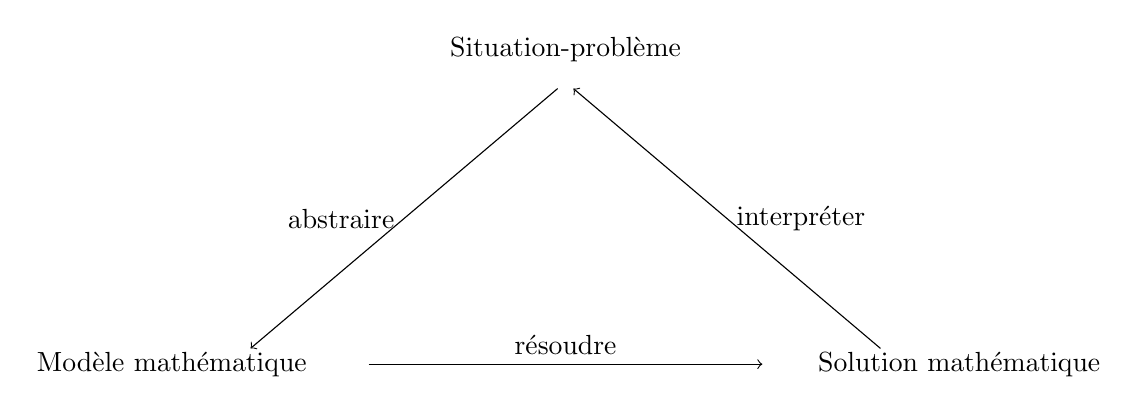
\begin{tikzpicture}
\draw (0,0) node {Situation-problème};
\draw[->] (-0.1,-0.5) -- (-4,-3.8) node[left,pos=0.5] {abstraire};
\draw (-5,-4) node {Modèle mathématique} ;
 \draw[->]
(-2.5,-4) -- (2.5,-4) node [above, pos=0.5] {résoudre};
\draw (5,-4)  node {Solution mathématique};
\draw[->] (4,-3.8) -- (0.1,-0.5)  node[right,pos=0.5] {interpréter};
\end{tikzpicture}
\end{myfig}

%\begin{mywrapfigsimp}{3.05in}{3.35in}
%\noindent
%\inputpdft{1-1-fig}
%\diffypdfversion{\par\vspace*{5pt}}
%\end{mywrapfigsimp}
Comment utilise-t-on les équations différentielles en science et en génie?  On commence avec une \emph{\myindex{situation-problème}} qu'on veut comprendre.  À l'aide d'hypothèses supplémentaires pour simplifier le problème, on crée un 
\emph{\myindex{modèle mathématique}}.  Autrement dit, on traduit la situation en équations différentielles.  Ensuite, on utilise les mathématiques afin d'obtenir une \emph{\myindex{solution mathématique}}.  Mais ce n'est pas fini.  Il faut encore interpréter les résultats: qu'est-ce que la solution mathématique nous dit à propos de la situation-problème de départ?

Pour ce qui est de formuler le modèle mathématique, et d'interpréter les résultats, vous ferez cela surtout dans vos cours de génie et de science.  Dans ce cours-ci, nous nous concentrerons principalement sur l'analyse mathématique.  Parfois, nous travaillerons avec des exemples réalistes simples afin de développer notre intuition et de motiver les concepts que nous verrons.

Considérons ici un exemple.  Une des équations les plus fondamentales est le \emph{\myindex{modèle de croissance exponentielle}}.  Dénotons une population de bactéries par la variable $P$ (plus précisément, $P$ dénote la quantité de population).  On suppose que l'environnement contient suffisamment de nutriments et d'espace.  Dans ce cas-là, le taux de croissance de la population de bactéries est proportionnelle à la population -- une population plus nombreuse cro\^itra plus rapidement.  Dénotons le temps (en secondes, disons) par la variable $t$.  Notre modèle est alors: 
%
\begin{equation*}
\frac{dP}{dt} = kP, 
\end{equation*}
où $k > 0$ est une constante.

\begin{example}
Supposons qu'il y a 100 bactéries au temps 0 et 200 bactéries 10 secondes plus tard.  Combien aura-t-on de bactéries à une minute (60 secondes) du début?

%mbxSTARTIGNORE
%mbxENDIGNORE
%
% Make sure to keep the above and the mbx figure below in sync!
%
D'abord, nous devons résoudre l'équation différentielle.  Nous affirmons que la fonction suivante est une solution: 
\begin{equation*}
P(t) = C e^{kt}, 
\end{equation*}
où $C$ est une constante.  Vérifions ceci: 
\begin{equation*}
\frac{dP}{dt} = C k e^{kt} = k P .
\end{equation*}
Il s'agit donc bel et bien d'une solution.

Ensuite?  On ne connaît pas la valeur de $C$, ni de $k$.  Mais on sait ceci: $P(0) = 100$ et $P(10) = 200$.  
Substituons ces valeurs dans l'expression et regardons ce que nous obtenons: 
\begin{align*}
& 100 = P(0) = C e^{k0} = C ,\\
& 200 = P(10) = 100 \, e^{k10} .
\end{align*}
Par conséquent, $2 = e^{10k}$ ou $\frac{\ln 2}{10} = k \approx 0,069$.
Donc: 
\begin{equation*}
P(t) = 100 \, e^{(\ln 2) t / 10} \approx 100 \, e^{0,069 t} .
\end{equation*}
à une minute, $t=60$, la population est $P(60) = 6400$.  
Voir la~\figurevref{intro:plotbactfig}.
%
\begin{myfig}
\capstart
\diffyincludegraphics{width=3in}{width=4.5in}{intro-plotbact}
\caption{Croissance de bactéries en 60 secondes.\label{intro:plotbactfig}}
\end{myfig}


%mbxlatex \begin{myfig}
%mbxlatex \capstart
%mbxlatex \diffyincludegraphics{width=3in}{width=4.5in}{intro-plotbact}
%mbxlatex \caption{Bacteria growth in the first 60 seconds.\label{intro:plotbactfig}}
%mbxlatex \end{myfig}

Parlons maintenant de l'interprétation de ces résultats.  Doit-on penser qu'il y aura exactement 6400 bactéries à 60 secondes? Bien sûr que non.  Nous avons fait des hypothèses simplificatrices qui ne seront pas exactement vraies, mais approximativement vraies.  Si nos hypothèses sont raisonnables, il y aura environ 6400 bactéries.  De plus, $P$ devrait être un nombre entier, puisqu'il compte une quantité de bactéries.  Pourtant, notre modèle admet des nombres comme $P(61) \approx 6859,35$.
%Obviously there 
%are either 6859 bacteria or 6860 bacteria.
\end{example}

Habituellement, la constante $k$ dans $P' = kP$ est connue, et l'on cherche à résoudre l'équation différentielle pour différentes \emph{conditions initiales\index{initial condition}}.  Qu'est-ce que \c{c}a veut dire?  Prenons $k=1$ pour simplifier les choses.  Supposons que nous voulons résoudre l'équation 
$\frac{dP}{dt} = P$ 
avec la condition $P(0) = 1000$ (la condition initiale).
Alors, la solution est (exercice): 
\begin{equation*}
P(t) = 1000 \, e^t .
\end{equation*}

On appelle $P(t) = C e^t$ \emph{la \myindex{solution générale}},
puisque toute solution de l'équation peut s'écrire sous cette forme pour un certain choix de la constante $C$.  La condition initiale sert à déterminer $C$, afin de trouver la 
\emph{\myindex{solution particulière}}.  
%Generally, when we say \myquote{particular solution,} we just mean some solution.

\subsection{Quatre équations fondamentales} \label{subsection:fourfundamental}

Quelques équations apparaissent fréquemment, et nous pouvons trouver utile de tout simplement apprendre par c{\oe}ur leur solution (nous les verrons aussi de manière plus formelle dans les chapitres suivants)  Appelons-les nos \myindex{quatre équations fondamentales}. Leurs solutions sont assez simples à deviner en nous rappelant les propriétés des exponentielles, de sinus et de cosinus.  Elles sont aussi plutôt simples à vérifier, ce qu'on devrait toujours faire.  Comme \c{c}a, inutile de se demander si on s'est rappelé correctement de la solution.

\medskip

Voici notre première équation fondamentale: 
\begin{equation*}
	\frac{dy}{dx} = k y,
\end{equation*}
où $k > 0$ est une constante.
Ici, $y$ est la variable dépendante, et $x$, la variable indépendante.
La solution générale de cette équation est: 
\begin{equation*}
	y(x) = C e^{kx} .
\end{equation*}
Nous avons vu ceci dans l'exemple précédent de la croissance exponentielle, même si les noms de variables ont changé.

\medskip

La deuxième équation s'obtient en modifiant légèrement
 la première: 
\begin{equation*}
	\frac{dy}{dx} = -k y,
\end{equation*}
où $k > 0$ est une constante.
La solution générale de cette équation est: 
\begin{equation*}
	y(x) = C e^{-kx} .
\end{equation*}

\begin{exercise}
Vérifiez que $y$ est bien une solution à cette équation.
\end{exercise}

Notre troisième équation fondamentale est une 
\emph{\myindex{équation différentielle du second ordre}}: 
\begin{equation*}
\frac{d^2y}{{dx}^2} = -k^2 y, 
\end{equation*}
où $k > 0$ est une constante.
La solution générale de cette équation est: 
\begin{equation*}
y(x) = C_1 \cos(kx) + C_2 \sin(kx) .
\end{equation*}
Puisque l'équation est du second ordre, la solution contient deux constantes.

\begin{exercise}
	Vérifiez que $y$ est bien une solution à cette équation.
\end{exercise}

Enfin, considérons l'équation suivante, elle aussi du second ordre: 
\begin{equation*}
	\frac{d^2y}{{dx}^2} = k^2 y ,
\end{equation*}
où $k > 0$ est une constante.
La solution générale de cette équation est: 
\begin{equation*}
	y(x) = C_1 e^{kx} + C_2 e^{-kx} 
\end{equation*}
ou
\begin{equation*}
	y(x) = D_1 \cosh(kx) + D_2 \sinh(kx) .
\end{equation*}

Les fonctions $\cosh$ and $\sinh$ se définissent comme suit:
\begin{equation*}
	\cosh x = \frac{e^{x} + e^{-x}}{2} , \qquad
	\sinh x = \frac{e^{x} - e^{-x}}{2} .
\end{equation*}
Elles s'appellent respectivement 
\emph{\myindex{cosinus hyperbolique}}
et
\emph{\myindex{sinus hyperbolique}}.
Elles sont parfois plus simples à utiliser que les fonctions exponentielles.  Elles ont de jolies propriétés, telles que
$\cosh 0 = 1$, $\sinh 0 = 0$, $\frac{d}{dx} \cosh x = \sinh x$ (non, il n'y a pas de signe \emph{moins}, ce n'est pas une coquille)
et $\frac{d}{dx} \sinh x = \cosh x$.

\begin{exercise}
	Vérifiez que les deux expressions sont des solutions à cette équation.
\end{exercise}

\begin{example}
	Pour les équations d'ordre supérieur, les solutions comportent plus de constantes pour lesquelles on doit résoudre afin d'obtenir une solution particulière.  L'équation  $\frac{d^2y}{dx^2} = 0$ a pour solution générale $y = C_1 x + C_2$; il suffit d'intégrer deux fois, sans oublier les constantes d'intégration.  Considérons les conditions initiales $y(0) = 2$ et $y'(0) = 3$.  On substitue ces valeurs dans la solution et l'on obtient: 
	\begin{equation*}
		2 = y(0) = C_1 \cdot 0 + C_2 = C_2, \qquad
		3 = y'(0) = C_1 .
	\end{equation*}
	Ainsi, $y = 3x + 2$ est la solution particulière recherchée.
\end{example}

Fait intéressant à propos de $\cosh$:  le graphe de $\cosh$ est précisément la forme d'une cha\^inette pendante (pas d'une parabole, contrairement à ce qu'on pourrait croire).  Cette forme s'appelle une \emph{\myindex{caténaire}}.
De plus, le graphe de $\cosh$ offre la forme idéale pour une arche supportant son propre poids; une telle arche de forme parabolique risquerait de s'écrouler. Un exemple célèbre est la  Gateway Arch de la ville américaine de Saint-Louis, dont la formule est inscrite dans la structure:
\begin{equation*}
	y = -127,7 \; \textrm{pi} \cdot \cosh({x / 127,7  \; \textrm{pi}}) + 757,7 \;\textrm{pi} .
\end{equation*}


\subsection{Exercices}

\begin{exercise}
	Montrez que $x = e^{4t}$ est une solution de $x'''-12 x'' + 48 x' - 64 x = 0$.
\end{exercise}

\begin{exercise}
	Montrez que $x = e^{t}$ n'est pas une solution de $x'''-12 x'' + 48 x' - 64 x = 0$.
\end{exercise}

\begin{exercise}
	Est-ce que $y = \sin t$ est une solution de ${\left( \frac{dy}{dt} \right)}^2 = 1 - y^2$?
	Justifiez votre réponse.
\end{exercise}

\begin{exercise}
Considérons $y'' + 2y' - 8y = 0$.  
Essayez une solution de la forme $y = e^{rx}$ pour une constante (à déterminer) $r$.  Existe-il une valeur de $r$ qui donne une solution? Si oui, trouvez toutes les valeurs possibles de $r$.
\end{exercise}

\begin{exercise}
Vérifiez que $x = C e^{-2t}$ est une solution de $x' = -2x$.
Trouvez $C$ satisfaisant la condition initiale $x(0) = 100$.
\end{exercise}

\begin{exercise}
	Vérifiez que $x = C_1 e^{-t} + C_2 e^{2t}$ est une solution de $x'' - x' -2 x =
	0$.  Trouvez $C_1$ and $C_2$ satisfaisant les conditions initiales $x(0) = 10$
	et $x'(0) = 0$.
\end{exercise}

\begin{exercise}
	Trouvez une solution
	${(x')}^2 + x^2 = 4$
	en utilisant ce que vous avez appris à propos des dérivées dans vos cours de calcul.
\end{exercise}

\begin{exercise}
	Résolvez 
	\begin{tasks}(2)
		\task $\dfrac{dA}{dt} = -10 A, \quad A(0)=5$
		\task $\dfrac{dH}{dx} = 3 H, \quad H(0)=1$
		\task $\dfrac{d^2y}{dx^2} = 4 y, \quad y(0)=0, \quad y'(0)=1$
		\task $\dfrac{d^2x}{dy^2} = -9 x, \quad x(0)=1, \quad x'(0)=0$
	\end{tasks}
\end{exercise}

\begin{exercise}
	Existe-t-il une solution de $y' = y$, telle que $y(0) = y(1)$?
\end{exercise}

\begin{exercise}
	La population de la ville X était 100 000 il y a 20 ans, et 120 000 il y a 10 ans.  Si on suppose une croissance continue, on peut utiliser le modèle de croissance exponentielle (comme pour une population de bactéries).  À combien estimez-vous la population actuelle maintenant?
\end{exercise}

\begin{exercise}
	Supposons qu'un coach de football obtient présentement un salaire annuel de 1 million $\$$, et qu'il a une augmentation salariale de $10\%$ chaque année (donc modèle de croissance exponentielle, comme les bactéries).  Dénotons par $s$ le salaire en millions de dollars, et $t$ le temps en années.
	\begin{tasks}(2)
	\task Trouvez $s(0)$ et $s(1)$.
	\task Après combien d'années approximativement le salaire sera-t-il de 10 millions?
	\task Après combien d'années approximativement le salaire sera-t-il de 20 millions?
	\task Après combien d'années approximativement le salaire sera-t-il de 30 millions?
	\end{tasks}
\end{exercise}


%mbxSTARTIGNORE
\noindent
\emph{Note: Les exercices dont les numéros sont 101 et plus ont des réponses à la fin du manuel.}
%mbxENDIGNORE

%mbx <p><em>Note: Exercises with numbers 101 and higher have solutions.</em></p>

\setcounter{exercise}{100}

\begin{exercise}
	Montrez que $x = e^{-2t}$ est une solution de $x'' + 4x' + 4x = 0$.
\end{exercise}
\exsol{%
	Calculer $x' = -2e^{-2t}$ et $x'' = 4e^{-2t}$.  Alors
	$(4e^{-2t}) + 4 (-2e^{-2t}) + 4 (e^{-2t}) = 0$.
}

\begin{exercise}
	Est-ce que $y = x^2$ est une solution de $x^2y'' - 2y = 0$?  Justifiez votre réponse.
\end{exercise}
\exsol{%
	Oui.
}

\begin{exercise}
	Soit $xy'' - y' = 0$.  Essayez une solution de la forme $y = x^r$.  Existe-t-il une valeur de $r$ qui donne une solution?  Si oui, trouvez toutes les valeurs possibles de $r$.
\end{exercise}
\exsol{%
	$y=x^r$ est une solution pour $r=0$ et $r=2$.
}


\begin{exercise}
Vérifiez que $x=C_1e^t+C_2$ est une solution de $x''-x' = 0$.  Trouvez $C_1$ et 
$C_2$ telles que $x(0) = 10$ et $x'(0) = 100$.
\end{exercise}
\exsol{%
$C_1 = 100$, $C_2 = -90$
}

\begin{exercise}
	Résolvez $\frac{d\varphi}{ds} = 8 \varphi$ and $\varphi(0) = -9$.
\end{exercise}
\exsol{%
	$\varphi = -9 e^{8s}$
}

\begin{exercise}
	Résolvez
	\begin{tasks}(2)
	\task $\dfrac{dx}{dt} = -4x, \quad x(0)=9$
	\task $\dfrac{d^2x}{dt^2} = -4x, \quad x(0)=1, \quad x'(0)=2$
	\task $\dfrac{dp}{dq} = 3 p, \quad p(0)=4$
	\task $\dfrac{d^2T}{dx^2} = 4 T, \quad T(0)=0, \quad T'(0)=6$
	\end{tasks}
\end{exercise}
\exsol{%
	a)~$x=9e^{-4t}$ \quad
	b)~$x=\cos(2t)+\sin(2t)$ \quad
	c)~$p=4e^{3q}$ \quad
	d)~$T=3\sinh(2x)$
}

%%%%%%%%%%%%%%%%%%%%%%%%%%%%%%%%%%%%%%%%%%%%%%%%%%%%%%%%%%%%%%%%%%%%%%%%%%%%%%

\sectionnewpage
\section{Classification des équations différentielles}
\label{classification:section}

%%Perhaps no [EP] ref?
%\sectionnotes{less than 1 lecture or left as reading\BDref{, \S1.3 in \cite{BD}}}
Il y a plusieurs types d'équations différentielles, et on les classifie en différentes catégories selon leurs propriétés.  Parlons brièvement d'une classification de base.  D'abord, la distinction entre EDO et EDP:
\begin{itemize}
\item
	Dans les \emph{équations différentielles ordinaires}\index{Équations différentielles ordinaires}\index{EDO}, ou EDO, les dérivées sont prises par rapport à une seule variable.  Autrement dit, il y a une seule variable indépendante.

\item
	Dans les \emph{équations aux dérivées partielles}\index{Équations aux dérivées partielles}\index{EDP}, ou EDP, les dérivées sont prises par rapport à plusieurs variables.  Autrement dit, il y a plusieurs variables indépendantes.
\end{itemize}

Voici quelques exemples d'équations différentielles ordinaires:
\begin{align*}
	& \frac{d y}{dt} = ky  & & \text{(croissance exponentielle\index{exponential growth})} \\
	& \frac{d y}{dt} = k(A-y)  & & \text{(\myindex{loi de refroidissement de Newton})} \\
	& m \frac{d^2 x}{dt^2} + c \frac{dx}{dt} + kx = f(t) . & &
\text{(vibrations mécaniques\index{mechanical vibrations})}
\end{align*}
Voici quelques exemples d'équations aux dérivées partielles:
\begin{align*}
	& \frac{\partial y}{\partial t} + c \frac{\partial y}{\partial x} = 0 & & 
		\text{(équation du transport\index{Équation du transport})} \\
	& \frac{\partial u}{\partial t} = \frac{\partial^2 u}{\partial x^2}  & & 
		\text{(équation de la chaleur ou de la diffusion\index{Équation de la chaleur/diffusion})} \\
	& \frac{\partial^2 u}{\partial t^2} = \frac{\partial^2 u}{\partial x^2} + \frac{\partial^2 u}{\partial y^2} . & & 
		\text{(équation de l'onde en 2 dimensions\index{Équation de l'onde en deux dimensions})}
\end{align*}

Lorsque la situation est soumise à plusieurs équations en même temps, on a un
\emph{\myindex{système d'équations différentielles}}.  
Par exemple: 
\begin{equation*}
	y' = x , \qquad x' = y
\end{equation*}
est un système simple d'équations différentielles ordinaires.
Les \myindex{équations de Maxwell} en électromagnétisme forment elles aussi un système d'équations aux dérivées partielles:
\begin{align*}
	& \nabla \cdot \vec{D} = \rho & & \nabla \cdot \vec{B} = 0  \\
	& \nabla \times \vec{E} = - \frac{\partial \vec{B}}{\partial t} &
	& \nabla \times \vec{H} = \vec{J} + \frac{\partial \vec{D}}{\partial t} .
\end{align*}
Les opérateurs de divergence $\nabla \cdot$ et de rotationnel $\nabla \times$ s'écrivent en termes de dérivées partielles des fonctions en termes des variables $x$, $y$ et $z$.

\medskip

Le prochain élément d'information est l'\emph{\myindex{ordre}} de l'équation (ou du système).   L'ordre est tout simplement l'ordre de la plus grande dérivée apparaissant dans l'équation.  Si la plus grande dérivée est la dérivée première, c'est une équation du premier ordre.  Si la dérivée la plus grande est la dérivée seconde, alors c'est une équation du deuxième ordre.  Par exemple, la loi de refroidissement de Newton est une équation du premier ordre, alors que l'équation des vibrations mécaniques est une équation du deuxième ordre.  L'équation décrivant les vibrations transversales dans une poutre, 
\begin{equation*}
	a^4 \frac{\partial^4 y}{\partial x^4} + \frac{\partial^2 y}{\partial t^2} = 0,
\end{equation*}
est une équation aux dérivées partielles d'ordre quatre.  En effet, une des dérivées dans l'équation est la quatrième dérivée.  Le fait que la dérivée en $t$ soit seulement d'ordre deux n'affecte pas l'ordre de l'équation.

Dans le premier chapitre, nous commencerons par les équations différentielles ordinaires du premier ordre, c'est-à-dire les équations de la forme $\frac{dy}{dx} = f(x,y)$.  En général, les équations de petit ordre sont plus simples à résoudre et à étudier.

\medskip

Dans la classification des équations, on s'intéresse aussi à comment les variables dépendantes apparaissent dans l'équation (ou le système).  En particulier, on l'appelle une 
\emph{équation linéaire}\index{linear equation} si la variable dépendante (ou les variables dépendantes) et ses dérivées apparaissent linéairement,  c'est-à-dire qu'elles ne sont pas multipliées ensemble et qu'aucune autre fonction des variables dépendantes n'apparaît dans l'équation.  Sinon, il s'agit d'une équation 
\emph{non linéaire}\index{nonlinear equation}.  Une EDO est linéaire si elle peut être exprimée de la manière suivante: 
\begin{equation} \label{classification:eqlingen}
a_n(x) \frac{d^n y}{dx^n} 
	+ a_{n-1}(x) \frac{d^{n-1} y}{dx^{n-1}} 
	+ \cdots
	+ a_{1}(x) \frac{dy}{dx} 
	+ a_{0}(x) y 
	= b(x) *.
\end{equation}
Les fonctions $a_0$, $a_1$, \ldots, $a_n$ s'appellent les
\emph{\myindex{coefficients}}.
L'équation peut dépendre arbitrairement de la variable indépendante.  Ainsi, l'équation suivante est linéaire:
\begin{equation} \label{classification:eqlinex}
	e^x \frac{d^2 y}{dx^2} + \sin(x) \frac{d y}{dx} +  x^2 y = \frac{1}{x},
\end{equation}
et ce, malgré la présence de $e^x$ et de $\sin(x)$, puisque $y$ et ses dérivées apparaissent de manière linéaire dans l'équation.

Tous les exemples mentionnés au début de la section sont linéaires.  Ce n'est peut-être pas évident dans le cas des équations de Maxwell; pour s'en convaincre, on peut écrire la divergence et le rotationnel en termes des dérivées partielles. 

Considérons maintenant quelques équations non linéaires.  Par exemple, l'équation de \myindex{Burger}, 
\begin{equation*}
	\frac{\partial y}{\partial t} +  \frac{\partial y}{\partial x} 
	= \nu \frac{\partial^2 y}{\partial x^2}, 
\end{equation*}
est une EDP du second ordre, qui est non linéaire, puisque $y$ et $\frac{\partial y}{\partial x}$ sont multipliés ensemble.
L'équation suivante: 
\begin{equation} \label{classification:eqnonlinode}
	\frac{dx}{dt} = x^2,
\end{equation}
est une EDO non linéaire du premier ordre, puisque la variable dépendante $x$ est au carré.

\medskip

Une équation qui est linéaire est de plus appelée \emph{\myindex{homogène}} si tous les termes dépendent de la variable dépendante.  Autrement dit, il n'y a aucun terme qui dépend uniquement de la variable indépendante.  Sinon, l'équation est dite \emph{\myindex{non homogène}}.  Par exemple, l'équation de la croissance exponentielle, l'équation de l'onde et l'équation du transport sont homogènes.  L'équation des vibrations mécaniques est non homogène à moins que $f(t)$ soit la fonction nulle.  De manière analogue, la loi de refroidissement de Newton est non homogène sauf si la température ambiante $A$ est nulle.
Une EDO linéaire homogène peut être écrite sous la forme suivante: 
\begin{equation*}
a_n(x) \frac{d^n y}{dx^n} 
	+ a_{n-1}(x) \frac{d^{n-1} y}{dx^{n-1}} 
	+ \cdots
	+ a_{1}(x) \frac{dy}{dx}
	+ a_{0}(x) y = 0 .
\end{equation*}
Comparez à \eqref{classification:eqlingen} et observez l'absence de fonction $b(x)$.

\medskip

Lorsque les coefficients d'une équation linéaire sont en fait des constantes, on dit alors que l'équation est à 
\emph{coefficients constants}\index{constant coefficient}.
Les coefficients sont les fonctions multipliées par la variable dépendante ou par une de ses dérivées, et non la fonction $b(x)$ qui appara\^it seule.
Une EDO non homogène à coefficients constants a la forme suivante: 
\begin{equation*}
	a_n \frac{d^n y}{dx^n} 
		+ a_{n-1} \frac{d^{n-1} y}{dx^{n-1}} 
		+ \cdots
		+ a_{1} \frac{dy}{dx}
		+ a_{0} y 
		= b(x), 
\end{equation*}
où $a_0, a_1, \ldots, a_n$ sont toutes des constantes, mais 
où $b$ peut dépendre de la variable indépendante $x$.
L'équation des vibrations mécaniques que nous avons vue plus haut est une EDO non homogène du second ordre à coefficients constants.  

La même nomenclature s'applique aux EDP.  Par conséquent, les équations du transport, de la chaleur/diffusion et de l'onde sont toutes des EDP linéaires à coefficients constants.

\medskip

Pour terminer, une équation est dite \emph{\myindex{autonome}}
 si l'équation ne dépend pas de la variable indépendante.  Pour des EDO autonomes, on pensera souvent à la variable indépendante comme à la variable du temps.  être une équation autonome signifie que l'équation ne varie pas dans le temps.  Par exemple, la loi de refroidissement de Newton est autonome, ainsi que l'équation \eqref{classification:eqnonlinode}.  Par contre, les équations de vibrations mécaniques ou \eqref{classification:eqlinex} ne sont pas autonomes.

\subsection{Exercices}

\begin{exercise}
	Classifiez les équations suivantes. S'agit-il d'une EDO ou d'une EDP?  Est-ce une équation ou un système?  Quel est l'ordre?  Est-ce linéaire ou non-linéaire et si c'est linéaire, est-ce homogène? à coefficients constants?  Si c'est une EDO, est-elle autonome?
	\begin{tasks}(2)
	\task $\displaystyle \sin(t) \frac{d^2 x}{dt^2} + \cos(t) x = t^2$
	\task $\displaystyle \frac{\partial u}{\partial x} + 3 \frac{\partial u}{\partial y} = xy$
	\task $\displaystyle y''+3y+5x=0, \quad x''+x-y=0$
	\task $\displaystyle \frac{\partial^2 u}{\partial t^2} + u\frac{\partial^2 u}{\partial s^2} = 0$
	\task $\displaystyle x''+tx^2=t$
	\task $\displaystyle \frac{d^4 x}{dt^4} = 0$
	\end{tasks}
\end{exercise}

\begin{exercise}
Si $\vec{u} = (u_1,u_2,u_3)$ est un vecteur, sa divergence est:
$\nabla \cdot \vec{u} =
	\frac{\partial u_1}{\partial x} 
	+ \frac{\partial u_2}{\partial y} 
	+ \frac{\partial u_3}{\partial z}$ et son rotationnel est: 
	$\nabla \times \vec{u} =
		\Bigl(	\frac{\partial u_3}{\partial y} - \frac{\partial u_2}{\partial z} , ~
				\frac{\partial u_1}{\partial z} - \frac{\partial u_3}{\partial x} , ~
				\frac{\partial u_2}{\partial x} - \frac{\partial u_1}{\partial y} \Bigr)$.
Observez que le rotationnel d'un vecteur est lui-même un vecteur.  écrivez les équations de Maxwell en termes de dérivées partielles et classifiez le système.
\end{exercise}

\begin{exercise}
	Supposons que $F$ est une fonction linéaire, c'est-à-dire que $F(x,y) = ax+by$ pour des constantes $a$ et $b$.  Classifiez les équations de la forme $F(y',y) = 0$.
\end{exercise}

\begin{exercise}
	Trouvez un exemple explicite d'un système de deux EDO satisfaisant les critères suivants: d'ordre trois, non autonome, non homogène, dont les coefficients sont non constants, et tel que toutes les dérivées possibles apparaissent dans le système au moins une fois.
\end{exercise}

\setcounter{exercise}{100}

\begin{exercise}
	Classifiez les équations suivantes. S'agit-il d'une EDO ou d'une EDP?  Est-ce une équation ou un système?  Quel est l'ordre?  Est-ce linéaire ou non-linéaire et si c'est linéaire, est-ce homogène? à coefficients constants?  Si c'est une EDO, est-elle autonome?
	\begin{tasks}(2)
	\task $\displaystyle \frac{\partial^2 v}{\partial x^2} + 3 \frac{\partial^2 v}{\partial y^2} = \sin(x)$
	\task $\displaystyle \frac{d x}{dt} + \cos(t) x = t^2+t+1$
	\task $\displaystyle \frac{d^7 F}{dx^7} = 3F(x)$
	\task $\displaystyle y''+8y'=1$
	\task $\displaystyle x''+tyx'=0, \quad y''+txy = 0$
	\task $\displaystyle \frac{\partial u}{\partial t} = \frac{\partial^2 u}{\partial s^2} + u^2$
	\end{tasks}
\end{exercise}
\exsol{%
	a) EDP\@, équation, deuxième ordre, linéaire, non homogène, coefficients constants. \\
	b) EDO\@, équation, premier ordre, linéaire, non homogène, coefficients non constants, non autonome.\\
	c) EDO\@, équation, ordre sept, linéaire, homogène, coefficients constants, autonome.\\
	d) EDO\@, équation, deuxième ordre, linéaire, non homogène, coefficients constants, autonome.\\
	e) EDO\@, système, deuxième ordre, non linéaire.\\
	f) EDP\@, équation,  deuxième ordre, non linéaire.
}

\begin{exercise}
	Écrivez la forme générale de l'équation différentielle ordinaire d'ordre \emph{zero} et linéaire.  Trouvez sa solution générale.
\end{exercise}
\exsol{%
	équation: $a(x) y = b(x)$, solution: $y = \frac{b(x)}{a(x)}$.
}

\begin{exercise}
	Pour quelles valeurs de $k$ l'équation $\frac{dx}{dt}+x^k = t^{k+2}$ est-elle linéaire?  Indice: il y a deux valeurs possibles.
\end{exercise}
\exsol{%
	$k=0$ ou $k=1$
}
